\section{Sistemas de V�deo \label{sistemas_de_video}}

Os sistemas de v�deo consistem na organiza��o em que uma determinada
informa��o de v�deo � armazenada em forma digital, tais como AVI,
MPEG, entre outros. O MPEG (Movie Pictures Experts Group) � um
padr�o internacional definido pela ISO que tem como caracter�stica a
compress�o de um v�deo. Onde, ao comprimir uma determinada amostragem
de um v�deo, o mesmo � passado pelo canal compressor, e ao exibir
esta mesma amostragem o v�deo passa pelo canal expansor (Figura \ref{img_mpeg}).

\begin{figure}[h|top]
 \centering
 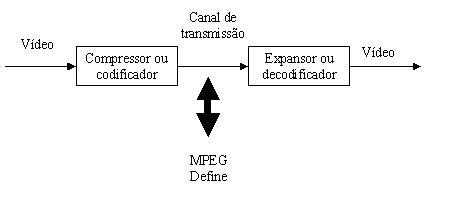
\includegraphics[width=1.0\linewidth]{imagens/mpeg.png}
 \caption{Sistema de Codifica��o e Decodifica��o de um v�deo no formato MPEG.}
 \label{img_mpeg}
\end{figure}


Audio Video Interleave, o AVI � um padr�o criado pela Microsoft em
1992, formato derivado do padr�o RIFF (Resource Interchange File
Format), o qual divide os dados em blocos. Ao contr�rio dos outros
padr�es o AVI n�o possui compress�o, resultando em arquivos com
tamanhos grandes, por�m, sem perda de qualidade. Na Figura
\ref{img_avi} observa-se que, da direita para a esquerda, a
estrutura de dados de um arquivo AVI primeiramente � formado pelo
cabe�alho RIFF, onde seus respectivos componentes s�o: tamanho do
arquivo total, bloco de dados ou lista de bloco de dados. Quando o
bloco de dados � definido em sub-blocos, cada parte � identificado
pelo ID e em seguida o tamanho do sub-bloco correspondente.

\begin{figure}[h|top]
 \centering
 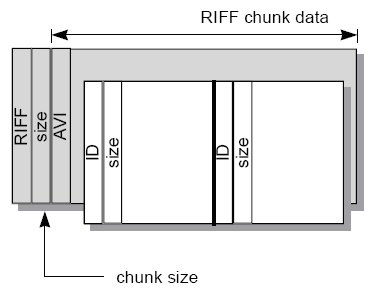
\includegraphics[width=0.8\linewidth]{imagens/avi.png}
 \caption{Sistema de armazenamento AVI.}
 \label{img_avi}
\end{figure}
